%---------------------------------------------------------------------------------------------------
% file: spojity_model_elmag_p.tex
%==============================Kapitola: Spojité matematické modely jednotlivých polí ==============
\chapter{Spojité matematické modely polí}
\minitoc
\newpage
  \section{Elektrický náboj}
    \subsection{Vlastnosti elektrického náboje}
      Na základě pokusů s elektřinou víme, že některá tělesa (například skleněná či ebonitová tyč
      po předchozím tření) mohou za určitých podmínek silově působit na jiná tělesa. Toto silové
      působení se vysvětluje přítomností elektrických nábojů. Elektrický náboj představuje pro nás
      výchozí fyzikální veličinu, přičemž mírou jejího množství a rozložení na příslušných tělesech
      je právě silové působení mezi nimi. Elektrický náboj je veličinou skalární, podobně jako
      hmotnost, a k jeho určení postačí jediná (reálná) číselná hodnota. Skutečnost, že síly
      elektrického působení mezi tělesy mohou být jak přitažlivé, tak odpudivé vysvětlujeme tím, že
      elektrický náboj může nabývat kladných i záporných hodnot - tělesa se souhlasným znamením
      náboje se přitom odpuzují, tělesa s nesouhlasným znamením náboje se přitahují. Tělesa, která
      nesou elektrický náboj nazýváme \emph{kladně} či \emph{záporně nabitá}, tělesa o nulovém
      náboji jsou elektricky \emph{neutrální}, nenabitá. Často se setkáváme s případem, kdy na
      tělesech jsou odděleně rozloženy kladné a záporné elektrické náboje o téže absolutní hodnotě.
      Taková tělesa budou také elektricky silově působit, přestože jejich celkový elektrický náboj
      je nulový. Říkáme jim \emph{polarizovaná}.
      
      O přítomnosti elektrického náboje se přesvědčujeme pouze na základě jeho silového projevu.
      Znamená to, že existenci jednoho jediného náboje bychom nemohli nijak odhalit. Kdyby
      existovaly pouze dva náboje, mohli bychom určit, zda jsou souhlasného či nesouhlasného
      znamení, nemohli bychom však rozhodnout ani o znamení, ani o velikosti těchto nábojů. Teprve
      jsou-li k dispozici alespoň tři náboje, můžeme jeden z nich vybrat jako jednotkový a kladný a
      ze silového působení určit velikost a znamení druhých nábojů\footnote{Co je vlastní podstatou
      elektrického náboje nevíme. Na základě poznatků současné mikrofyziky jej můžeme považovat za
      jednu z vlastností elementárních částic, která podmiňuje jejich vzájemné působení.
      Rozlišujeme čtyři základní typy vzájemného působení (\emph{interakce}) mezi elementárními
      částicemi: gravitační, slané elektromagnetické a silné. Gravitační interakce je univerzální a
      týká se všech částic. Setkali jsme se s ní v mechanice, její velikost udává Newtonův
      gravitační zákon a její podstatu se snaží objasnit obecná teorie relativity. Slabá interakce
      se projevuje u některých typů radioaktivního rozpadu za účasti neutrina. Podobně
      elektromagnetická interakce se uplatňuje mezi elementárními částicemi a jednou z jejích
      charakteristik je náboj. Silná interakce existuje mezi částicemi, které nazýváme hadrony, a
      drží pohromadě atomové jádro, které by se jinak odpudivými elektrickými silami působícími
      mezi protony musely rozdělit.
      
      Současný rozvoj mikrofyziky naznačuje, že hadrony, které jsme dříve považovali za
      elementární, mají svoji strukturu a komponenty. Předpokládáme o nich, že jsou tvořeny tzv.
      kvarky. Na současné úrovni vystupují tedy jako elementární kvarky a leptony (k nim patří
      elektron, mion, tauon a odpovídající neutrina), jejich antičástice a dále pak částice, které
      zprostředkovávají interakci mezi nimi}.
          
  \section{Elektromagnetické pole}       
    \subsection{Veličiny elektromagnetického pole a jejich jednotky}
      \fbox{Elektrický náboj} je \emph{skalární veličinou}. Jednotkou je \emph{coulomb [C]}. Má
         kvantový charakter (tj. je roven celistvému násobku elementárního náboje $e =
         1,602\cdot10^{-19}C$), avšak v technických aplikacích k tomu nepřihlížíme. Náboj $Q$
         může být rozložen:
         \begin{itemize}
            \item \emph{prostorově} v objemu $V$ s objemovou hustotou
               \begin{equation}\label{TEMP:eq_q_varrho}
                  \varrho = \frac{dQ}{dV} \qquad [C\cdot m^{-3}]
               \end{equation}               
            \item \emph{plošně} na ploše $S$, s plošnou hustotou
               \begin{equation}\label{TEMP:eq_q_sigma}
                  \sigma = \frac{dQ}{dS} \qquad [C\cdot m^{-2}]
               \end{equation}                 
            \item \emph{lineárně} na křivce $l$, s lineární hustotou
               \begin{equation}\label{TEMP:eq_q_tau}
                  \tau = \frac{dQ}{dl} \qquad [C\cdot m^{-1}]
               \end{equation}                 
         \end{itemize}
         Rozlišujeme:
           \begin{itemize}
             \item \textbf{volné náboje}: mohou se přemisťovat v makroskopických
             vzdálenostech,
             \item \textbf{vázané náboje}: mohou se přemisťovat jen v
             mikroskopických vzdálenostech.
           \end{itemize}
         Volnými náboji jsou volné elektrony v kovech nebo ionty v elektrolytech (jsou odpoutány od
         atomů, resp. molekul a volně se mezi nimi pohybují); vázané náboje vznikají polarizací
         dielektrika.
         
      \fbox{Elektrický proud}\label{TEMP:kap_el_proud_velicina} je znám z každodenního života,
        přesto je velmi důležité umět tento pojem vnímat jak pro označení „jevu“ (kap.
        \ref{TEMP:kap_elproud_jev}), tak jako fyzikální veličinu, která tento jev kvantitativně
        popisuje (kap. \ref{TEMP:kap_el_proud_velicina} ). Elektrický proud je \emph{skalární
        fyzikální veličina} ozn. $I$ resp. $i$, jejíž jednotkou je základní jednotka soustavy SI:
        \emph{ampér} – [A]. V této soustavě jednotek je ampér definován na základě silových
        účinků mezi dvěma vodiči, kterými prochází elektrický proud. Tato síla je magnetického
        původu, avšak magnetické pole vzniká jako důsledek pohybu elektrického náboje.Je tvořen
        uspořádaným pohybem elektrických nábojů.
        
        Připojíme-li vodič ke zdroji elektrického napětí, elektrické pole uvnitř působí elektrickou
        silou na vodivostní elektrony, vyvolává jejich pohyb a tím vytváří elektrický proud, který
        je po krátké době \emph{stacionární} (ustálený, nezávislý na čase). Jestliže vodičem projde
        náboj $\Delta Q$ resp. $dQ$ za časový interval $\Delta t$ resp. $dt$, lze definovat
        \emph{průměrný} resp. \emph{okamžitý} proud ve vodiči:
        \begin{itemize}
          \item \textbf{průměrný} elektrický proud: $$I_{AV} = \frac{\Delta Q}{\Delta t}
                \qquad[A],$$
          \item \textbf{okamžitý} elektrický proud (který je limitním případem proudu průměrného,
                studujeme-li množství náboje, které projde průřezem vodiče za infinitezimální
                (nekonečně krátký) časový interval): $$i = \lim_{\Delta t \rightarrow 0}\frac{\Delta
                Q}{\Delta t} = \frac{dQ}{dt} \qquad[A].$$ V ustáleném stavu protéká všemi průřezy
                vodiče stejně velký proud,
          \item speciálně pohybuje-li se náboj vodičem rovnoměrně, nazýváme proud
                \textbf{stejno\-směr\-ným}, $I(t) = \text{konst}$, a platí $$ I_{DC} =
                \frac{Q}{t}\qquad[A] $$
        \end{itemize}        

        Elektrický proud jako \emph{jev} charakterizuje jednu z forem fyzikálního pohybu, kterou je
        \textbf{uspořádaný pohyb elektricky nabitých částic} v látce. Přestože jakýkoliv elektrický
        proud je vždy tvořen pohybujícími se náboji, nemusí všechny pohybující se náboje vytvářet
        elektrický proud. Ve vodiči dochází ke vzniku trvalého elektrického proudu za těchto
        podmínek:
          \begin{itemize}
            \item vodič se musí nacházet v trvalém elektrickém poli, což je realizováno pomocí tzv.
                  \emph{zdroje} (generátoru) elektrického napětí,
            \item ve vodiči musí být přítomny volné nosiče elektrického náboje.
          \end{itemize}
        
        Podle charakteru vnějšího elektrického pole lze rozlišit tři základní druhy proudů:
          \begin{labeling}{stejnosměrný}
            \item[\textbf{stejnosměrný}] proud vzniká tehdy, jestliže má intenzita elektrického pole
                   konstantní orientaci,
            \item[\textbf{střídavý}] proud ve vodiči vytváří vnější elektrické pole, jehož intenzita
                  periodicky mění svou orientaci na opačnou,
            \item[\textbf{stacionární}] stejnosměrný proud vzniká ve vodiči, je-li intenzita
                  elektrického pole konstantní co do velikosti, směru i orientace.
          \end{labeling}  

       Nabité částice představující volný náboj ve vodičích jsou v neustálém chaotickém tepelném
       pohybu (viz molekulová fyzika a termodynamika). Jedná se o \emph{mikroskopický pohyb}, který
       nemá za následek makroskopicky pozorovatelné přemístění náboje. Pokud ve vodiči vytvoříme
       elektrické pole, tepelný pohyb nabitých částic neustane, ale k náhodné složce rychlosti
       přibude ještě složka rychlosti ve směru vloženého pole.
       
       Při studiu elektrického proudu v kovových vodičích se zabýváme ustálenými proudy
       vodivostních elektronů, které v kovu vytváří tzv. \emph{elektronový plyn}. Tyto vodivostní
       elektrony jsou téměř volné a pohybují se v poli kladných iontů uspořádaných v krystalové
       mřížce.
        
       Experimentálně lze elektromagnetické pole prokázat silovým působením na elektricky nabité
       částice. Celkovou sílu $\vec{F}$ lze rozložit na elektrickou sílu $\vec{F}_e$, nezávislou na
       tom, zda je nabitá částice v klidu nebo v pohybu vůči vztažné soustavě a na magnetickou sílu
       $\vec{F}_m$, působící jen na pohybující se částice. Elektromagnetické pole má tedy dvě
       složky: \textbf{elektrické pole}, působící na náboj silou $\vec{F}_e$ a \textbf{magnetické
       pole}, působící na pohybující se náboj silou $\vec{F}_m$  \cite[s.~13]{Mayer2001}.
        
      \fbox{Intenzita elektrického pole} $\vec{E}$ je vektorovou veličinou charakterizující
        \emph{elektrické pole}.
        Je definována jako 
        \emph{síla působící na nepohybující se jednotkový bodový náboj}:
        \begin{equation}\label{TEMP:eq_E}
          \vec{E} = \frac{\vec{F}_e}{Q} \qquad\left[\frac{V}{m}\right]  
        \end{equation}        
        kde $\vec{F}_e$ je elektrická síla působící na náboj $Q$.
                 
      \fbox{Magnetická indukce} $\vec{B}$ je vektorovou veličinou charakterizující \emph{magnetické
        pole}. Je definovována vztahem
        \begin{equation}\label{TEMP:eq_B}
          \vec{F}_m = Q(\vec{v}\times\vec{B}) \qquad[T]  
        \end{equation}        
        kde $\vec{F}_m$ je magnetická síla působící na náboj $Q$ pohybující se rychlostí $\vec{v}$.
        Jednotkou je \emph{tesla} $[T]$.
    
        Síla, jež působí elektromagnetické pole na pohybující se náboj se nazývá \textbf{Lorentzova
        síla}
         \begin{equation}\label{TEMP:eq_Lorentz}
          \vec{F} = \vec{F}_e + \vec{F}_m =Q(\vec{E} + \vec{v}\times\vec{B}) \qquad[N]  
        \end{equation}        

    \subsection{Maxwellovy rovnice}
      Makroskopická teorie elektromagnetického pole v klasickém pojetí vychází ze základních zákonů
      vyjádřených \emph{Maxwellovými rovnicemi (MR)}. Lze je zapsat buď v \textbf{integrálním},
      nebo \textbf{diferenciálním tvaru}. V integrálním tvaru popisují elektromagnetické pole v
      jisté prostorové oblasti $\Omega$, kdežto v diferenciálním tvaru ve vnitřním bodě této
      oblasti. Soustavu vlastních MR představují první čtyři páry rovnic; často se k nim připojuje
      jako další základní rovnice elektromagnetického pole rovnice kontinuity pro vodivý proud.
      Její integrální a diferenciální tvar reprezentují poslední dvě rovnice.

      \begin{align}
        \oint_\mathcal{C}\vr{H} d\vr{l} &= I+\der{\Psi}{t}
                                           \quad \rot{H}=\vr{J}+\pder{\vr{D}}{t}             \\
        \oint_\mathcal{C}\vr{E} d\vr{l} &=& -\der{\Phi}{t}
                               \qquad \rot{E}=-\pder{\vr{B}}{t}\\
         \int_\mathcal{S}\vr{D} d\vr{S} &= Q \qquad\quad\;   \diver{D}=\rho_V                \\
         \int_\mathcal{S}\vr{B} d\vr{S} &= 0 \qquad\quad\;\; \diver{B}=0                     \\
         \int_\mathcal{S}\vr{J} d\vr{S} &= -\der{Q}{t} \qquad\diver{J}=-\der{\rho_V}{t}
      \end{align}

      Předpokládá se, že \emph{všechny křivky a plochy v integrálním tvaru MR jsou po částech
      hladké a všechny integrované veličiny jsou po částech spojité funkce}. Pak je zaručena
      existence integrálů v těchto rovnicích. V diferenciálním tvaru MR se předpokládají pouze
      \textbf{regulární body} oblastí, což jsou body, v nichž jsou veličiny $\vr{E}$, $\vr{D}$,
      $\vr{B}$ a $\vr{H}$ \emph{spojité a spojitě diferencovatelné funkce}; nejsou jimi tedy např.
      body rozhraní dvou různých prostředí, v elektrickém poli body v nichž jsou umístěny diskrétní
      náboje, v magnetickém poli body proudových vláken atd.

  \section{Elektrostatické pole}
    Zdrojem elektrostatického pole jsou elektrické náboje. Náboje se nepohybují (tj. nedochází k
    elektrickému proudu) a tedy nevzniká magnetické pole. Základní rovnice elektrostatické pole
    jsou:
    \begin{table}[h]
      \centering
      \catcode`\-=12
      \begin{tabular}{l c|c|}
        \cline{2-3}
        \multicolumn{1}{l|}{} & \textbf{integrální tvar} & \textbf{diferenciální tvar}  \\
        \hline
        \multicolumn{1}{|l|}{2. MR} & $\oint\vr{E}\cdot d\vr{l} = 0$ & $\rot{E} = 0$    \\ 
        \cline{1-3}
        \hline
        \multicolumn{1}{|l|}{3. MR} & $\oint\vr{D}\cdot d\vr{S} = Q$ & $\rot{D} = \rho$ \\
        \cline{1-3}
        & & $\vr{D} = \varepsilon\vr{E}$ \\
        \cline{3-3}
      \end{tabular}
      \caption{Základní rovnice elektrostatického pole}
   \end{table}

  % ----------------Stacionární magnetické pole-----------------------------------------------------  
  \newpage
  \section{Stacionární proudové pole}
    V elektrostatice (tj. elektrickém poli nepohybujících se nábojů) neexistuje trvalý elektrický
    proud. Zdroje napětí (galvanické články, termočlánky, dynama aj.) mají tu vlastnost, že na
    jejich záporné svorce je trvale nadbytek elektronů, a na jejich kladné svorce jejich
    nedostatek. Těmito zdroji můžeme ve vodiči trvale udržovat elektrické pole a tedy i tok nosičů
    elektřiny. Jestliže se \emph{náboje pohybují konstantní rychlostí, hovoříme o stacionárním
    elektrickém proudu}. Základní rovnice elektrostatické pole jsou:

    \begin{table}[ht!]
      \centering
      \catcode`\-=12
      \begin{tabular}{l c|c|}
        \cline{2-3}
        \multicolumn{1}{l|}{} 
          & \textbf{integrální tvar} & \textbf{diferenciální tvar}             \\
        \hline
        \multicolumn{1}{|l|}{2. MR} 
          & $\oint\vr{E}\cdot d\vr{l} = 0$ & $\rot{E} = 0$                     \\ 
        \cline{1-3}
        \hline
        \multicolumn{1}{|l|}{Zákon kontinuity} 
          & $\oint\vr{J}\cdot d\vr{S}=0$ & $\diver{J}=0$                       \\
        \cline{1-3}
        \multicolumn{1}{|l|}{Ohmův zákon} 
          & $I=GU=\frac{U}{R}$ & $\vr{J} =\gamma\vr{E} = \frac{1}{\rho}\vr{E}$ \\
        \cline{1-3}
      \end{tabular}
      \caption{Základní rovnice stacionárního proudového pole}
    \end{table}
    
    \subsection{Elektrický proud v kovových vodičích}\label{TEMP:kap_elproud_jev}
      V předchozí kapitole \ref{TEMP:kap_el_proud_velicina} bylo o elektrickém proudu pojednáváno
      jako o skalární fyzikální veličině. V této kapitole nás bude zajímat makroskopický pohled na
      „jev“ známý jako \emph{elektrický proud}.
      
      Zopakujme, že elektrickým proudem je míněn uspořádaný pohyb elektrických ná\-bo\-jů, a aby se
      tyto náboje mohly pohybovat, musí být volné - jsou přítomny v látkách, které nazýváme
      \textbf{vodiče}. Vodiče mohou mít nositele náboje jednoho znaménka (elektrony v kovech,
      uhlíku a v polovodičkých) anebo obojích znamének (kladné a záporné ionty v elektrolytech,
      ionty a elektrony v ionizovaných plynech). Volné nositele náboje (elektrony, ionty) lze
      rovněž oddělit od těchto látek (vodičů) a vytvořit elektrický proud ve vakuu nebo ve
      zředěných plynech.
      
      Z vodičů mají největší význam \textbf{kovy}, které jsou polykrystalickými látkami s kovovou
      vazbou. Každý mikroskopický monokrystal kovu má pevnou krystalovou mříž sestavenou z kladných
      iontů, mezi nimiž se přetržitě pohybují \emph{volné elektrony} rychlost\-mi, jejichž velikost
      je statisticky proměnná (co do veliskosti i směru). Střední hodnota rychlosti (jako vektoru)
      všech elektronů je nulová. Střední hodnota rychlosti určitého elektronu je závislá na teplotě
      vodiče. Elektrony konají tzv. \emph{termický pohyb}. Rychlosti neuspořádaných termických
      pohybů dosahují jen o několik řádů větších hodnot, než kmity iontů v krystalech mřížky.

      \begin{figure}
        \centering
        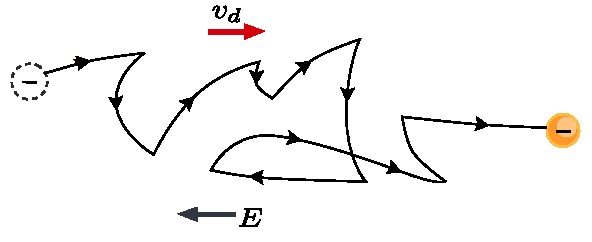
\includegraphics[width=\linewidth]{vd_e_drift.pdf}
        \caption[Pohyb elektronu ve vodiči.]{Pohyb elektronu ve vodiči. Fyzikálně je $v_d$ 
                 průměrná rychlost nosičů náboje uvnitř vodiče, který je vložen do vnějšího
                 elektrického pole. Ve skutečnosti se ale elektron ve vodiči nepohybuje po přímce,
                 jeho pohyb je chaotický.}
        \label{TEMP:fig_vd_e_drift}
      \end{figure}       
      
      Připojíme-li vodič k vnějšímu zdroji elektrického pole (např. ke galvanickému článku), začne
      statisticky převládat uspořádaný pohyb nosičů kladného (záporného) náboje ve směru (proti
      směru) vnějšího pole nad termickým pohybem, což v makroskopickém měřít\-ku pozorujeme jako
      \textbf{makroskopický elektrický proud}. Jsou-li ve vodiči přítomny nosiče náboje obou
      polarit, dojde k pohybu ve vzájemně opačných směrech, přičemž směr toku nosičů kladného
      náboje se historicky ztotožňuje se směrem toku elektrického proudu. U kovových vodičů je tedy
      směr proudu právě opačný, než směr toku elektronů, jenž tento elektrický proud tvoří.
      
      Velikost (intenzitu) proudu posuzujeme podle velikosti náboje obojí polarity, který projde
      určitým průřezem vodiče ve vzájemně opačných směrech za jednotku času. Projde-li průřezem
      vodiče celkově náboj $dQ$ za čas $dt$, bude tok náboje vodičem charakterizovat skalární
      veličina
        \begin{equation}\label{TEMP:eq_I_01}
          I = \frac{dQ}{dt} \qquad[A],  
        \end{equation}        
      která se nazývá \emph{elektrický proud}($1C\cdot s^{-1} = 1A $ čteno \emph{ampér}). Tato
      jednotka patří mezi základní jednotky \texttt{SI} soustavy.
      
      Pro \emph{stacionární} (tj. časově neproměnný - ustálený) proud můžeme obecný výraz
      \ref{TEMP:eq_I_01} nahradit rovnicí
        \begin{equation}\label{TEMP:eq_I_02}
          I = \frac{Q}{t}.  
        \end{equation}       
      Jedná-li se o rovnoměrný pohyb bodového náboje $Q$ po kružnici s periodou $T$, resp. s
      úhlovou rychlostí $\omega$, můžeme vzniklý ustálený proud vyjádřit rovnicí 
        \begin{equation}\label{TEMP:eq_I_03}
          I = \frac{Q}{T} = \frac{\omega Q}{2\pi}.  
        \end{equation}
      
      Bude-li se element náboje $dQ$ pohybovat v lineárním útvaru rychlostí $v = \frac{dQ}{dl}$,
      bude po dosazení do rov.\ref{TEMP:eq_I_01} reprezentovat elektrický proud 
        \begin{equation}\label{TEMP:eq_I_04}
          I = \frac{dQ}{dt} = \frac{dQ}{dl}v = \tau v, 
        \end{equation}      
      kde $\tau$ je \emph{délková hustota} náboje a $v$ je velikost \emph{okamžité rychlosti}
      náboje v uvažovaném místě lineárního útvaru. 

      \begin{figure}[ht!]
         \centering
         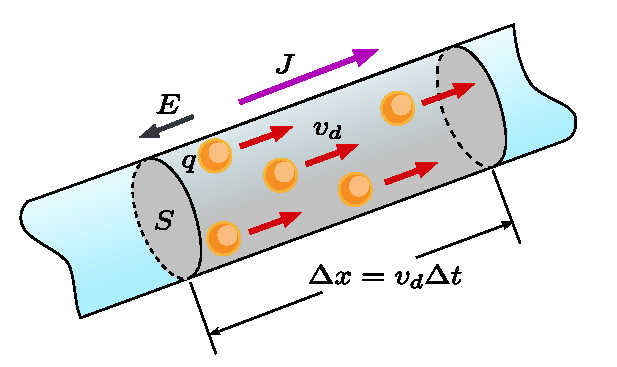
\includegraphics[width=0.9\linewidth]{el_proud_ve_vodici.pdf}
         \caption[Náboje, pohybující se vodičem]{Směr elektrického proudu byl implicitně stanoven
                  jako směr pohybu kladných nábojů. Nositeli elektrického náboje uvnitř vodičů jsou
                  ovšem záporně nabité volné elektrony, které se tedy dle  konvence pohybují proti
                  směru elektrického proudu. Elektrický proud může protékat pevnými látkami (kovy,
                  polovodiči), kapalinami (elektrolyty) a ionizovanými plyny. Látky, které nevedou
                  elektrický proud, nazýváme nevodiči, izolanty}
         \label{TEMP:fig_el_proud_ve_vodici}
      \end{figure}
      
      Elektrický proud je veličina, která obecně popisuje prostorový jev. Omezíme se nyní na běžný
      případ vodiče, jako je na obr. \ref{TEMP:fig_el_proud_ve_vodici}, který má volné náboje jen
      jedné polarity (u kovových vodičů jde o elektrony) a označme $\rho_0$ prostorovou hustotu
      volného náboje a $v_d$ velikost usměrněné rychlosti jejich nositelů (elektronů). Pak za čas
      $dt$ projde průřezem o obsahu $S_0$ ($S_0\bot v_d$) náboj $dQ = \rho_0 S_0 v_d dt$.
      Elektrický proud vyjádřený rov.
      \ref{TEMP:eq_I_01} můžeme přepsat do tvaru
        \begin{equation}\label{TEMP:eq_I_05}
          I = \rho_0 S_0 v_d = - e n_0 S_0 v_d, 
        \end{equation}         
      kde $\displaystyle{n_0 = \frac{\rho_0}{-e}}$ je počet nositelů volného náboje (tj. v našem
      případě elektronů, z nichž každý nese náboj $-e$ v jednotkovém objemu vodiče, přičemž pro
      elektrony zřejmě je $\rho_0<0$.

      \begin{figure}
        \centering
        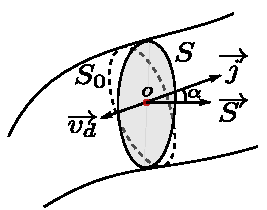
\includegraphics[width=0.8\linewidth]{plocha_S.pdf}
        \caption[Rovinná plocha $S$.]{Rovinná plocha $S = S_0\cos\alpha$}
        \label{TEMP:fig_plocha_S}
      \end{figure}           
      Rovinnou plochou $S$ průřezu můžeme zavést jako vektor $vr{S}$, který má směr daný normálou k
      ploše a pravidlem pravé ruky (ukazují-li prsty pravé ruky směr oběhu po hraniční křivce
      plochy, ukáže palec směr plochy jako vektoru $\vr{S}$). Protože driftová rychlost $v_d$ je
      také vektor, nebudeme obecně uvažovat vektory $\vr{S}, \vr{v_d}$ o stejném směru a rovnici
      \ref{TEMP:eq_I_05} přepíšeme do obecnějšího tvaru               
        \begin{equation}\label{TEMP:eq_I_06}
          I = \rho_0 \vr{S_0}\cdot\vr{v}_d = jS\cos\alpha = jS_0, 
        \end{equation}      
      kde $S_0 = S$ pro $\alpha = 0$ (viz obr. \ref{TEMP:fig_plocha_S}) a   
        \begin{equation}\label{TEMP:eq_I_07}
          \vr{j} = \rho_0\vr{v_d}, 
        \end{equation}        
      je proudová hustota. Je to vektor o velikosti 
        \begin{equation}\label{TEMP:eq_I_08}
          j = \frac{I}{S\cos\alpha} = \frac{I}{S_0}  \qquad A\cdot m^{-2}, 
        \end{equation}   
      obecněji
        \begin{equation}\label{TEMP:eq_I_09}
          j = \frac{dI}{dS}, 
        \end{equation}

      a o směru vektoru driftové rychlosti nositelů kladného náboje. Pro případ nositelů volného
      náboje - elektronů má proudová hustota opačný směr než driftová rychlost $v_d$ (obr.
      \ref{TEMP:fig_plocha_S}).
      
      Velikost vektoru $\vr{j}$ má význam plošné hustoty elektrického proudu v uvažovaném místě
      průřezu. Jednotkou je $A\cdot m^{-2}$.
      
      Nebude-li proudová hustota na uvažovaném průřezu konstantní, bude celkový elektrický proud
      procházející průřezem o obsahu $S$ dán integrálem 
        \begin{equation}\label{TEMP:eq_I_10}
          I = \int_S \vr{j}d\vr{S}. 
        \end{equation} 
     
      %---------- Driftová rychlost elektroknů ve vodiči:   
      \begin{example} \emph{Driftová rychlost elektronů ve vodiči:} Vodičem z jednomocné mědi o
        průřezu $S_0 = 1\ mm^2$ prochází elektrický proud $I = 5\ A$. Vypotěte:
          \begin{itemize}
            \item počet volných elektronů v jednotkovém objemu Cu,
            \item úhrný náboj volných elektronů v jednotkovém objemu,
            \item driftovou rychlost volných elektronů při proudu $I$.
          \end{itemize}
        Měd má poměrnou atomovou hmotnost $A_r = 63,54$ a hustotu\footnote{Pro hustotu budeme
        používat alternativní značku $s$, s ohledem na kolizi značky $\rho$, jež označuje hustotu
        náboje.} $s = 8,93\cdot10^3\ kg\cdot m^{-3}$.
       
       \textbf{Řešení:}\newline
         \begin{itemize}
           \item Jeden mol mědi o molové hmotnosi $M = 0,06354\ kg\cdot mol^{-1}$ a o molovém
                 objemu $$V_m = \frac{M}{s} = \frac{63,54\cdot10^{-3}\ kg\cdot
                 mol^{-1}}{8,93\cdot10^3\ kg\cdot m^{-3}} = 7,12\cdot10^{-6}\ m^3\cdot mol^{-1}$$
                 obsahuje $N_A = 6,0221\cdot10^{23}$ jednoatomových molekul \emph{Cu} na jeden mol,
                 z nichž každý má volný jeden (valenční) elektron. Tedy počet volných elektronů v
                 jednotkovém objemu je $$n_0 = \frac{N_A}{V_m} = \frac{sN_A}{M} =
                 \frac{6,0221\cdot10^{23}\ mol^{-1}}{7,12\cdot10^{-6}\ m^{3}\cdot mol^{-1}} =
                 8,46\cdot10^{28}\ m^{-3}.$$
           \item Úhrnný náboj volných elektronů v jednotkovém objemu mědi je $$Q_v = -e\cdot n_0 =
                 -1,36\cdot10^{10}\ Cm^{-3}.$$
           \item Velikost driftové rychlosti určíme ze vztahu $I = -en_0v_dS_0 = - Q_v v_d S_0$ tj.
                 $$v_d = \left|\frac{I}{Q_v S_0}\right| =
                 \frac{5}{1,36\cdot10^{10}\cdot1\cdot10^{-6}}\frac{C\cdot s^{-1}}{Cm^{-3}\cdot m^2}
                 = 3676\cdot10^{-4}\ \frac{m}{s} = 0,3676\ \frac{mm}{s}.$$
         \end{itemize}
         Z provedených výpočtů si můžeme udělat názor o mikroskopických poměrech v kovových
         vodičích: počet volných nositelů náboje - elektronů a jejich úhrný náboj v jednotkovém
         objemu je značný a proto driftová rychlost elektronů potřebná k vyvolání proudu běžné
         velikosti v drátových vodičích je nesmírně malá (doslova hlemýždí).
      \end{example}  
     
      \begin{example}
        Elektricky neutrální měděná mince o hmotnosti $ m = 3,11\ g$ obsahuje stejné množství
        kladného a záporného náboje. Jaké je velikost kladného (nebo záporného) náboje obsaženého v
        minci?
       
        \textbf{Řešení:}\newline
        Neutrální atom má záporný náboj $Z\cdot e$, představovaný jeho elektrony a kladný náboj o
        stejné velikosti představovaný protony v jádře. Pro měd je atomové číslo $Z$ rovno 29, tj.
        atom mědi má 29 protonů, a je-li elektricky neutrální, také 29 elektronů.
       
        Náboj o velikosti $Q_v$, který hledáme je roven $NZ_e$, kde $N$ je počet atomů obsažených v
        jednom molu (Avogadrova konstanta: $N_A = 6,0221\cdot10^{23}\ mol^{-1}$). Počet molů mědi v
        minci $\frac{m}{M}$, kde $M = 63,5\ g\cdot mol^{-1}$ je molární hmotnosti mědi:
        $$N = N_A\cdot\frac{m}{M} = 6,0221\cdot10^{23}\ mol^{-1}\frac{3,11\ g}{63,5\ g\cdot
        mol^{-1}} = 2,95\cdot10^{22}.$$ Velikost celkového kladného (záporného) náboje v minci je
        pak $$Q_v = NZ_e = 2,95\cdot10^{22}\cdot29\cdot1,602\cdot10^{-19}\ C = 137039\ C$$
        To je obrovský náboj. Pro srovnání: třeme-li ebonitovou tyč vlněnou látkou, můžeme na tyč
        přemístit stěží náboj o velikosti $10^{-9}\ C$.
      \end{example} 
 
    % ----------------Práce a výkon elektrického proudu---------------------------------------------
    \subsection{Práce a výkon elektrického proudu}
      \begin{example}
        Za jakou dobu uvede ponorný vodič o příkonu $600\ W$ do varu $1\ l$ vody o počáteční
        teplotě $20°C$. Uvažujte měrnou teplenou kapacitu vody $c = 4200\ J\cdot kg^{-1}\cdot
        K^{-1}$. Výměnu tepla s okolím neuvažujte. \newline \textbf{Řešení:}\newline
        Pro var vody bude zapotřebí tepla dle rovnice $Q  = m\cdot c\cdot(T_2 - T_1)$. Potřebná
        elektrická práce je $Q_e = P\cdot t = U\cdot I\cdot t$ a tedy dobu ohřevu stanovíme z
        rovnice:
          \begin{align*}
            P\cdot t &= m\cdot c\cdot(T_2 - T_1)               \\
                   t &= \frac{m\cdot c}{P}\cdot(T_2 - T_1)     \\
                   t &= \frac{1\cdot 4200}{600}\cdot(100 - 20) \\
                   t &= 560\ s
          \end{align*}         
      \end{example}
 
    % ----------------Ohmův zákon-------------------------------------------------------------------
    \subsection{Ohmův zákon}
      Uvažujme vodič u něhož jsou volnými nositeli náboje \emph{elektrony}. Nyní v mezích klasické
      mechaniky kvantitativně popíšeme mechanismus vedení proudu, který povede k všeobecně známému
      \textbf{Ohmovu zákonu}
      
      Umístíme-li vodič do elektrického pole o intenzitě $\vec{E}$ (např. připojením ke
      galvanickému článku), působí na každý volný elektron síla $\vec{F} = -e\vec{E}$, která mu
      podle \emph{Newtonova zákona} udělí zrychlení $\vec{a} = \frac{\vec{F}}{m_e} = -
      \frac{e}{m_e}\vec{E}$ proti směru vnějšího pole. Tím získávají chaoticky se pohybující
      elektrony ještě složku rychlosti v protisměu vloženého elektrického pole $\vec{E}$ a  dojde
      tedy k usměrnění driftového pohybu volných elektronů a v souladu s kapitolou
      \ref{TEMP:kap_elproud_jev} pozorujeme, že ve vodiči vznikl makroskopický elektrický proud.
      
      Pohyb elektronu se ovšem neobejde bez sřážek s ionty v krystalové mřížce. Dráhu, kterou se
      elektronu podaří urazit, nazýváme \emph{volnou dráhou} $d$. Průměrná doba mezi dvěma po sobě
      jdoucími srážkami nechť je $\tau$ za tuto dobu se bude elektron rovnoměrně urychlovat a těsně
      před následující srážkou jeho rychlost dosáhne maxima tj. $\vec{v}_{max} = \vec{a}\cdot\tau$.
      Nás ovšem zajímá průměrná rychlost (\emph{driftová rychlost})na volné dráze průměrné
      velikosti:
      \begin{equation}\label{TEMP:eq_vd_01}
        \vec{v}_d = \frac{\vec{v}_{max}}{2} = -\frac{e\tau}{2m_e}\vec{E}
      \end{equation}   
      Proudová hustota \ref{TEMP:eq_I_07} bude
      \begin{equation}\label{TEMP:eq_j_02}
        \vec{j} = \rho_0\vec{v}_d= -en_0\vec{v}_d = -\frac{e^2n_0\tau}{2m_e}\vec{E}
      \end{equation}       
      Koeficient úměrnosti 
      \begin{equation}\label{TEMP:eq_g_03}
        \gamma = \frac{e^2n_0\tau}{2m_e}
      \end{equation}     
      je závislý na počtů nositelů (elektronů) $n_0$ v jednotkovém objemu a na době $\tau$, neboli
      na délce volné dráhy. Veličina $\gamma$ se nazývá \emph{měrná elektrická vodivost} neboli
      \textbf{konduktivita} látky. Protože dobu $\tau$ nelze přímo měřit, určuje se $\gamma$
      experimentálně. Přitom se zjišťuje, že pro určitou teplotu zkoumané látky je $\gamma$
      konstantí.
      
      Po zevedení pojmu měrná elektrická vodivost látky \ref{TEMP:eq_g_03}, můžeme výraz
      \ref{TEMP:eq_j_02} přepsat do výsledného tvaru
      \begin{equation}\label{TEMP:eq_j_04}
        \vec{j} = \gamma\vec{E},
      \end{equation}              
      který se v literatuře označuje jako \emph{Ohmův zákon v diferenciálním tvaru} (i když se v
      pravém slova smyslu o diferenciální tvar nejedná). Výstižnější je označení \emph{lokální tvar
      Ohmova zákona}, protože výraz \ref{TEMP:eq_j_04} se vztahuje na určité místo, resp. bod,
      vodivého prostředí. Vztah říká, že proudová hustota v určitém bodě vodivého prostředí je
      přímo úměrná intenzitě vloženého elektrického pole v tomto bodě (platí pro určitou teplotu
      prostředí).
      
      Uvažujme nyní lineární homogenní vodič délky $l$ a příčného průřezu o obsahu $S_0$, připojený
      ke zdroji o napětí $U$. Pak intenzita pole uvnitř vodiče bude mít konstantní velikost
      $E=\frac{U}{l}$. Dosadíme-li za velikost proudové hustoty $j=\frac{I}{S_0}$ do
      \ref{TEMP:eq_j_04}, dostaneme vztah
      \begin{equation}\label{TEMP:eq_j_05}
        \frac{I}{S_0} = \gamma\frac{U}{l},
      \end{equation}        
      z něhož vyplývá známý vztah
      \begin{equation}\label{TEMP:eq_j_06}
        U = \frac{l}{\gamma S_0}I = RI,
      \end{equation}              
      kde
      \begin{equation}\label{TEMP:eq_j_07}
        R = \frac{l}{\gamma S_0} = \rho\frac{l}{S_0},
      \end{equation} 
      je \textbf{elektrický odpor} uvažovaného lineárního vodiče, přičemž $\rho = \frac{1}{\gamma}$
      je \emph{měrný elektrický odpor} (\textbf{rezistivita})\footnote{Zde je další kolize značky
      $\rho$. Nyní se tomuto problému vyhneme využíváním pouze konduktivity, jenž se častěji
      používá v teorii elektromagnetického pole.}. Výraz \ref{TEMP:eq_j_07} představuje klasický
      Ohmův zákon zákon experimentálně objevený r. 1826 \emph{G. S. Ohmem}. Jednotky:
      \begin{itemize}
        \item elektrický odpor: \si{V.A^{-1}},
        \item měrný elektrický odpor: \si{\ohm.m},
        \item měrná elektrická vodivost: \si{\ohm^{-1}.m^{-1}}.
      \end{itemize}
      
      \begin{example}
        \textbf{Zemnicí elektroda}: Uvažujte zemnicí elektrodu ve tvaru koule o poloměru
        $a=\SI{200}{\mm}$, uloženou do zeminy v hloubce, která je značně větší než je poloměr $a$.
        Pro jednoduchost řešení dále předpokládejte, že přívodíní drát je od zeminy izolován (obr.
        \ref{TEMP:fig_zem_elektroda}). Zemina má měrnou vodivost $\gamma=\num[exponent-product =
        \cdot]{1,8e-2}\si{\per\ohm\per\m}$. Při zkratu teče přívodním drátem proud $I=\SI{50}{\A}$.
        Vypočítejte:

          %----------------------------------
          % image: TEMP_zem_elektroda.tex label: \label{TEMP:fig_zem_elektroda}
            % \documentclass{article}
% \usepackage{tikz}
% \usetikzlibrary{decorations.markings}
% \usetikzlibrary{intersections}
% \usetikzlibrary{calc}

% \begin{document}
  \begin{figure}
    \centering  
    \begin{tikzpicture}[scale=1, every node/.style={scale=1}]
      \coordinate (pCenter) at (0,-5);
      \fill[brown!60] (-2,-0.2) rectangle (2,-7);
      \draw[color=brown, line width=5pt] (-2,-0.2) -- +(4,0); 
      \draw[->,line width=1pt] (0,1) node[left] {$I$} -- (0,-0.1);        
      \draw[line width=1pt] (0,0) -- (pCenter);
      \draw[line width=1pt,color=black, fill=white]
           (pCenter) circle[radius=0.5];
      \draw[line width=1pt, dotted]
           (pCenter) circle[radius=1];
      \foreach \angle in
          {0, 30, 60, 120, 150, 180, 210, 240, 270, 300, 330}
      {
        \draw[->, line width=0.75pt] (pCenter)++(\angle:1.2) -- +(\angle:0.3);        
      }
      \draw[<->, thick] (pCenter)++(240:1) coordinate(pR) -- (pCenter) -- +(330:0.5) coordinate(pA); 
      \node[above] at ($ (pCenter)!0.5!(pA) $) {$a$};     
      \node[above] at ($ (pCenter)!0.9!(pR) $) {$r$}; 
      \node[above] at (-1,-2) {$\gamma$};
      \node[above] at (+1.5,-4.5) {$\vec{j}$};
    \end{tikzpicture}
    \caption{Zemnicí elektroda}\label{TEMP:fig_zem_elektroda}
  \end{figure}
  
% \end{document}    
          %----------------------------------         
        \begin{enumerate}[label=\emph{\alph*})]
          \item Závislost potenciálu $\varphi=\varphi(r)$ elektrického pole, které se vytvoří v
                zemině při zkratu, kde $r$ je vzdálenost od středu elektrody. Potenciál normujte
                volbou $\varphi(\infty)=0$.
          \item Zemnicí odpor elektrody, který je definován vztahem $$R_z=\frac{U_z}{I_z},$$ kde
                $U_z = \varphi(a)-\varphi(b)$ je zmnicí napětí 
          \item Ztrátový výkon při zkratu.            
        \end{enumerate}
        Řešení:    
        Ekvipotenciální a proudové plochy mají zřejmě kulový tvar se středem totožným s
        geometrickým středem elektrody. Proudová hustota na kulové ploše obecného poloměru $r$
        (viz. obr. \ref{TEMP:fig_zem_elektroda}) je $$\vec{j}=\frac{I}{4\pi r^2}\vec{n},$$ kde
        $\vec{n}$ je jednotkový vektor ve směru normály. Pak v bodech na této ploše musí být
        elektrické pole o intenzitě $\vec{E}$, kterou určíme ze vtzahu
        \begin{equation*}
         \vec{j}= \gamma\vec{E}\rightarrow\vec{E}=
                  \frac{\vec{j}}{\gamma}=\frac{I}{4\pi\gamma r^2}\vec{n}.
        \end{equation*}
        Závislost potenciálu $\varphi=\varphi(r)$ tohoto elektrického pole stanovíme pomocí
        následujícího integrálu
        \begin{equation}
          \varphi = - \int\vec{E}d\vec{r}+C = -\frac{I}{4\pi\gamma}\int\frac{dr}{r^2} + C 
                  =   \frac{I}{4\pi\gamma r} + C, \nonumber
        \end{equation} 
        kde integrační konstantu $C$ určíme z okrajové podmínky $\varphi(\infty)=0$, odkud $C=0$.
        Hledaná závislost potenciálu je
        \begin{equation*}
         \varphi = \frac{I}{4\pi\gamma r}, \qquad r\in\langle a, \infty). 
        \end{equation*}           
        
        Zemina, v níž je uložena elektroda, je vastně rezistorem, jehož jeden okraj tvoří elektrodu
        a druhým okrajem je nekonečně rozlehý vodivý prostor.
        Potenciální rozdíl mezi těmito okraji je
        \begin{equation*}
         U_z = \varphi(a) - \varphi(\infty)= \frac{I}{4\pi\gamma a},
        \end{equation*} 
        \begin{minipage}[t]{0.5\textwidth}% first column            
        odkud zemnicí odpor 
        \begin{equation*}
          R_z = \frac{U_z}{I} = \frac{I}{4\pi\gamma a} = \SI{22,1}{\ohm}
        \end{equation*}
        \end{minipage}
        \begin{minipage}[t]{0.5\textwidth}% second column    
        a ztrátový výkon 
        \begin{equation*}
          P_z = R_z\cdot I^2 = \SI{55,3}{\kilo\watt}. 
        \end{equation*}
        \end{minipage}
      \end{example}
      
    % ------------------- Elektromotorické napětí --------------------------------------------------
    \subsection{Elektromotorické napětí}
      Uzavřený proudový okruh $C$, nechť je v dynamické rovnováze - prochází jím ustálený
      elektrický proud. Uvažujme pro jednoduchost představy kladný náboj - ten se musí pohybovat ve
      směru klesajícího potenciálu (záporný náboj ve směru stoupajícího potenciálu). Je-li okruh
      uzavřený, musí kladné náboje opět vystoupit na místo s vyšším potenciálem - musí se tedy
      pohybovat proti elektrostatickým silám. Proto proti úbytku      
               
  % ----------------Stacionární magnetické pole-----------------------------------------------------
  \newpage
  \section{Stacionární magnetické pole}
    Zdrojem stacionárního magnetického pole jsou stejnosměrné proudy nebo permanentní magnety.
    Základní rovnice stacionárního magnetického pole jsou:

    \begin{table}[ht!]
      \centering
      \catcode`\-=12
      \begin{tabular}{l c|c|}
        \cline{2-3}
        \multicolumn{1}{l|}{} & \textbf{integrální tvar} & \textbf{diferenciální tvar} \\
        \hline
        \multicolumn{1}{|l|}{1. MR} & $\oint\vr{H}\cdot d\vr{l} = I$ & $\rot{H} = \vr{J}$ \\ \cline{1-3}
        \hline
        \multicolumn{1}{|l|}{4. MR} & $\oint\vr{B}\cdot d\vr{S} = 0$ & $\diver{B} = 0$ \\
        \cline{1-3}
        & & $\vr{B} = \mu \vr{H}$ \\
        \cline{3-3}
      \end{tabular}
      \caption{Základní rovnice magnetického stacionárního pole}
    \end{table}

    Směr vektoru $\vr{H}$ se prakticky určí například \emph{pravidlem pravotočivého šroubu}: vodič
    nahradíme šroubem (s pravotočivým závitem) a otáčíme jím tak, aby se pohyboval ve směru proudu;
    směr otáčení pak udává směr vektoru $\vr{H}$. Vše je názorně vysvětleno na obrázku
    \ref{temp:fig_pravidlo_sroub}. Podobných pomůcek existuje více, např. \emph{pravidlo pravé
    ruky}: vodič uchopíme do dlaně pravé ruky tak, aby palec ukazoval směr proudu; prsty pak
    ukazují směr vektoru $\vr{H}$, obr. \ref{temp:fig_pravidlo_ruka}.

         \begin{figure}[ht!]
           \centering
           \subfloat[Pravidlo pravé ruky]{\label{temp:fig_pravidlo_ruka}
             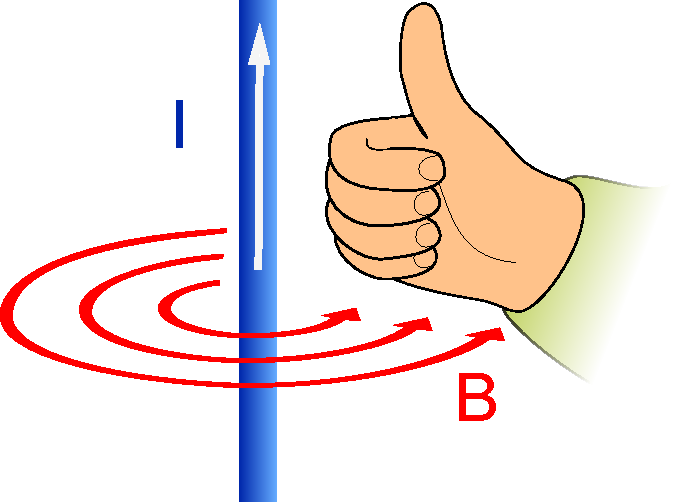
\includegraphics[width=0.5\linewidth]{pravidlo_prave_ruky.pdf}}
           \subfloat[Pravidlo pravotočivého šroubu]{\label{temp:fig_pravidlo_sroub}
             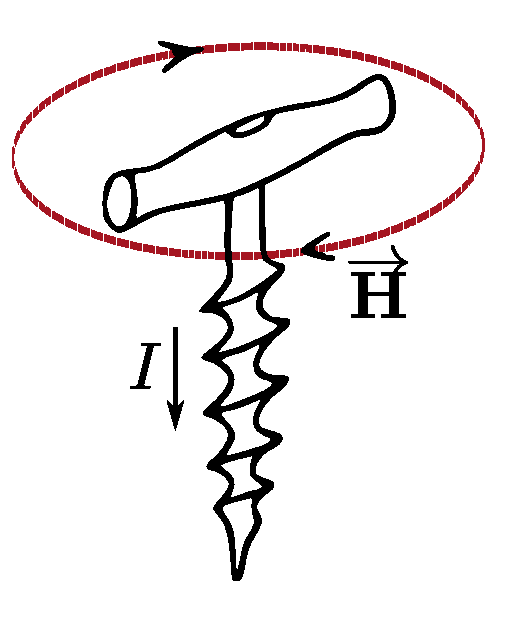
\includegraphics[width=0.4\linewidth]{pravidlo_pravotociveho_sroubu.pdf}}
           \caption[Pravidlo pravé ruku a pravotočivého šroubu]{Určení směru vektoru $\vr{H}$: a)
                   pravidlem pravé ruky; b) pravidlem pravotočivého šroubu}
           \label{temp:fig_urceni_H}
         \end{figure}
    K procvičení těchto pravidel je na obr. \ref{TEMP:fig_ind_c_kruh_z} vyznačen směr indukčních
    čar kruhové\-ho závitu. Označení $\bigotimes$ vyjadřuje proud vstupující  do nákresny (symbol
    letícího šípu od pozorovatele) a označením $\bigodot$ proud vystupující z nákresny (symbol
    hrotu šípu).
    
    \begin{wrapfigure}{r}{2.4in}
      \centering
      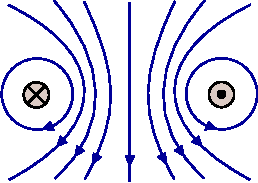
\includegraphics[width=0.2\textwidth]{mag_ind_cary_kruh_z.pdf}
      \caption{Indukční čáry kruhového závitu.}
      \label{TEMP:fig_ind_c_kruh_z}
    \end{wrapfigure}    
    Rovnice \ref{TEMP:eq_zak_celk_I} představuje \textbf{zákon celkového proudu} vyjadřující,
    rovnost oběhového magnetické napětí na libovolné uzavřené orientované křivce $c$ proudu, který
    je s křivkou $c$ spřažen. ''\emph{Spřaženým proudem}'' rozumíme proud, který prochází libovolnou
    plochou $S$, jež je ohraničená křivkou $c$, přičemž plocha $S$ je orientována vůči křivce $c$
    pravotočivě (obr. \ref{TEMP:fig_1MR_pic}). \cite[s.~55]{Mayer2001}.

      \begin{equation}\label{TEMP:eq_zak_celk_I}
        \oint\vr{H}\cdot d\vr{l} = I   
      \end{equation}    
     
      \begin{figure}[ht!]
         \centering
         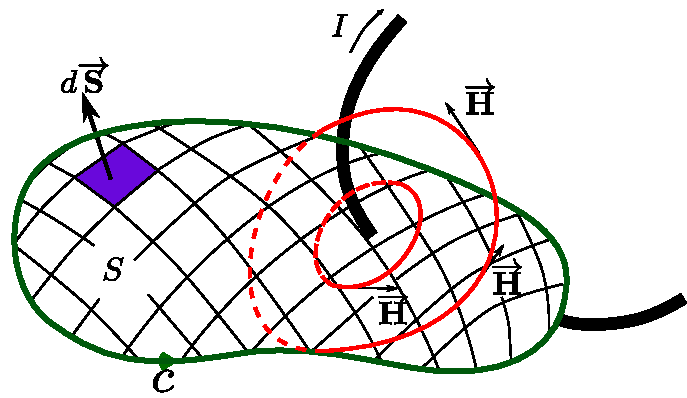
\includegraphics[width=\linewidth]{1MR_pic.pdf}
         \caption[Zákon celkového proudu]{K zákonu celkového proudu}
         \label{TEMP:fig_1MR_pic}
      \end{figure}

         \begin{figure}[hb!]
           \centering
           \subfloat[$\oint\vr{H}\cdot d\vr{l} = 0$]{\label{TEMP:fig_mag_sprazeny_proud1}
             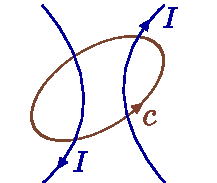
\includegraphics[width=0.3\linewidth]{mag_sprazeny_proud1.pdf}}
           \subfloat[$\oint\vr{H}\cdot d\vr{l} = 0$]{\label{TEMP:fig_mag_sprazeny_proud2}
             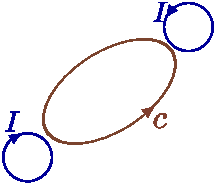
\includegraphics[width=0.3\linewidth]{mag_sprazeny_proud2.pdf}}
           \subfloat[$\oint\vr{H}\cdot d\vr{l} = 3I$]{\label{TEMP:fig_mag_sprazeny_proud3}
             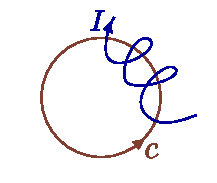
\includegraphics[width=0.3\linewidth]{mag_sprazeny_proud3.pdf}}             
           \caption[K pojmu ''proud spřažený s křivkoku'']{K pojmu ''proud spřažený s křivkoku''
                    pro tři různé případy křivky $c$.}
           \label{TEMP:fig_mag_sprazeny_proud123}
         \end{figure}
         
    Základní úlohou řešení stacionárních proudových magnetických polí je určení rozložení veličin $\vr{H}$ a 
    $\vr{B}$ v prostoru, je-li dáno prostorové a materiálové uspořádání a elektrické proudy vybuzují řešené 
    magnetické pole.
    
    V následujících úlohách se omezíme na analýzu jednodušších, souměrných magnetických polí v lineárním 
    izotropním alespoň po částech homogenním prostředí. Pro zjednodušení budeme zanedbávat deformaci 
    magnetického pole v okrajových oblastech a nebudeme uvažovat vliv blízkosti nesymetrického rozhraní a 
    vliv blízkosti druhého zdroje magnetického pole. (Pro přesnější řešení by pak bylo nutné použít tzv. 
    \emph{metodu zrcadlení}.) Některá složitější pole lze rozdělit na několik jednodušších polí souměrného 
    charakteru, resp. typického uspořádání. Vzhledem k tomu, že v předpokládaném lineárním prostředí ($\mu = 
    konst$) platí pro stacionární magnetické pole \emph{princip superpozice}, lze samostatně vyřešit nejpreve 
    dílčí jednodušší pole jednotlivých proudů $I_j$ a po jejich superpozici
      \begin{equation}\label{TEMP:eq_superp_mag_pole}
        \vr{H}= \sum_{j=1}^n\vr{H}_j(I_j), \quad\text{resp.}\quad \vr{B}= \sum_{j=1}^n\vr{B}_j(I_j)   
      \end{equation}
    získáme výsledné pole celkového proudu \cite[s.~181]{Kotlan1999}. 
    
    Metodou přímé aplikace I. Maxwellovy rovnice v integrálním tvaru pro stacionární magnetické
    pole proudové
      \begin{equation}\label{TEMP:eq_1MR_rozbor}
        \oint_\mathcal{C}\vr{H}d\vr{l} = \oint_\mathcal{C}H\cos\alpha dl = I_c
      \end{equation}    
    lze jednoduše použít tehdy, je-li ze zadané úlohy zřejmá taková symetrie pole, že lze z nekonečně mnoha 
    uzavřených křivek, splňující rov. \ref{TEMP:eq_1MR_rozbor}, nalézt takovou integrační dráhu $c$, která 
    obepíná proud $I_c$ vytvářející magnetické pole a v jejichž bodech platí podmínka
      \begin{equation}\label{TEMP:eq_H_alpha_konst}
        H = \text{konst}, \qquad \alpha = \text{konst},
      \end{equation}    
    speciálně
      \begin{equation}\label{TEMP:eq_alpha_0}
        H = \text{konst}, \qquad \alpha = 0.
      \end{equation}
    
    Podmínka $\alpha = 0$, tj. $\vr{H}\| d\vr{l}$ je identicky splněna na siločáře magnetického pole. 
    Siločáry souměrných stacionárních magnetických polí splňují tedy podmínku \ref{TEMP:eq_alpha_0} a řešení 
    rovnice \ref{TEMP:eq_1MR_rozbor} při integraci po takovéto siločáře je jednoduché
      \begin{equation}\label{TEMP:eq_1MR_alpha0}
        \oint_\mathcal{C}\vr{H}d\vr{l} = H\underbrace{\oint_\mathcal{C} dl}_{l_c} = 
                                         I_c \rightarrow H = \frac{I_c}{l_c}
      \end{equation}            
    kde $l_c$ je délka integrační dráhy $c$ splňující podmínku \ref{TEMP:eq_alpha_0}.
      
    Klasickým případem takovéto úlohy je magnetické pole \emph{dlouhého přímého válcového vodiče} o
    poloměru $a$, délky $l$ protékaného proudem $I$ rozloženým po průřezu souměrně kolem osy vodiče, tzn, 
    obecně s hustotou $J = J(r)$. Z osové (rotační) symetrie vyplývá, že siločáry magnetického pole mají 
    tvar soustředných kružnic se středem v ose vodiče, ležících v rovině kolmé na osu vodiče obr. 
    \ref{TEMP:fig_mag_pole_vodic_I_konst}.
    \begin{figure}[ht!]
      \centering
      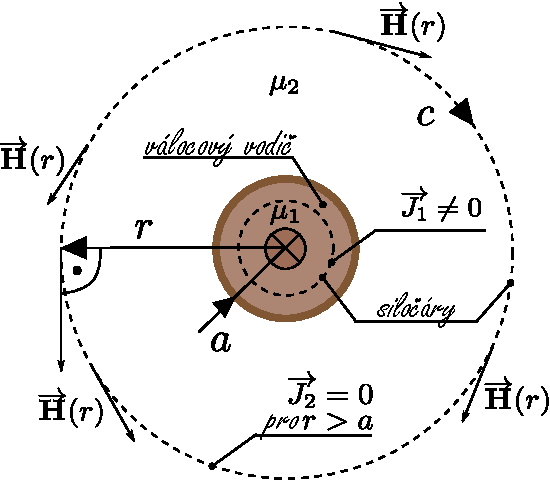
\includegraphics[width=0.9\linewidth]{mag_pole_vodic_I_konst.pdf}
      \caption[Pole dlouhého dutého vodiče protékaného konstantním proudem]{Pole dlouhého dutého
               vodiče protékaného konstantním proudem}
      \label{TEMP:fig_mag_pole_vodic_I_konst}
    \end{figure}        
    Úlohy proto řešíme ve válcových souřadnicích s osou $z$ totožnou s osou vodiče. Za předpokladu, že průměr 
    vodiče je zanedbatelný vůči jeho délce lze zanedbat deformaci pole vlivem konců válcového vodiče a přejít 
    na rovinný problém v polárních souřadnicích. Z důvodu osové souměrnosti je však pole závislé jen na 
    vzdálenosti $r$ od osy vodiče tj. $$H = H(r), \qquad B = B(r).$$ Na kruhových siločárách je tedy splněna 
    podmínka \ref{TEMP:eq_alpha_0} a z I. Maxwellovy rovnice \ref{TEMP:eq_1MR_rozbor} 
      \begin{equation}\label{TEMP:eq_1MR_rozbor2}
        \oint_{\mathcal{C}}\vr{H}d\vr{l} = H\cos0\oint_\mathcal{C}dl = I(r),
      \end{equation}     
    kde $c$ je kružnice o poloměru $r$ a proud $I(r)$ je dán rovnicí
      \begin{equation}\label{TEMP:eq_1MR_Ir}
        I(r) = \int_{S(r)}\vr{J}(r)d\vr{S} = \int_0^rJ(r)2\pi rdr
      \end{equation}           
    je proud protékající přes kruhovou plochu $S(r)$ ohraničenou kružnicí o poloměru $r$. Pak
    intenzita magnetického pole ve vzdálenosti $r$ od osy vodiče má velikost
      \begin{equation}\label{TEMP:eq_Hr_vodice}
        H = H(r) = \frac{I(r)}{2\pi r},
      \end{equation}       
    a magnetická indukce 
      \begin{equation}\label{TEMP:eq_Br_vodice}
        B = B(r) = \frac{\mu I(r)}{2\pi r},
      \end{equation}       
    přičemž $\mu$ je \emph{permeabilita} v bodech na poloměru $r$. Magnetické pole v okolí
    kruhové\-ho přímého vodiče protékaného proudem $I$ viz obr.
    \ref{TEMP:fig_mag_pole_vodic_I_konst_sol} je tedy v souladu s předchozími úvahami dáno výrazy   
    \cite[s.~183 - 185]{Kotlan1999}:
    \begin{figure}[ht!]
      \centering
      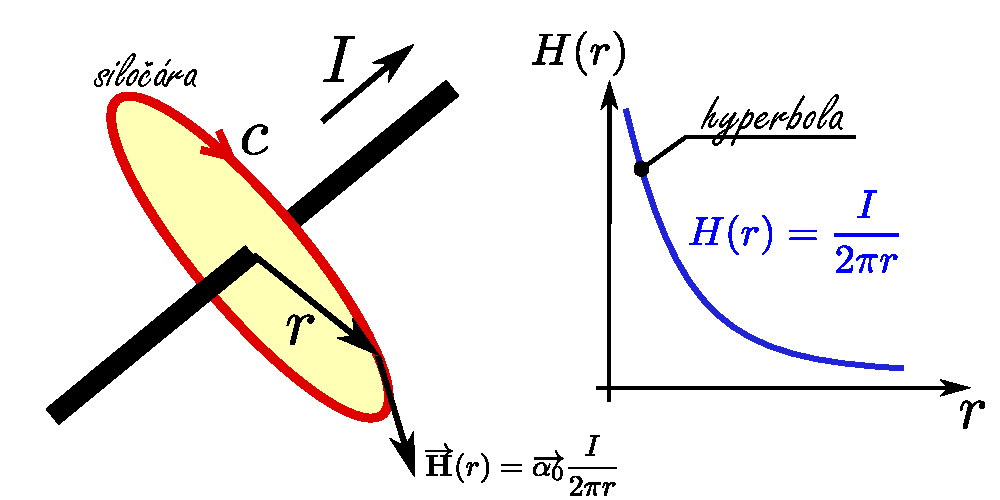
\includegraphics[width=0.9\linewidth]{mag_pole_vodic_I_konst_sol.pdf}
      \caption[Průběh intenzity magnetického pole dlouhého dutého vodiče protékaného konstantním
               proudem]{Průběh intenzity magnetického pole dlouhého dutého vodiče protékaného
               konstantním proudem}
      \label{TEMP:fig_mag_pole_vodic_I_konst_sol}
    \end{figure}      
      \begin{equation}\label{TEMP:eq_Hr_Br_vodice}
        H = H(r) = \frac{I}{2\pi r}, \qquad B = B(r) = \frac{\mu I}{2\pi r}.
      \end{equation}   
    Jelikož 1. MR má nenulovou pravou stranu v magnetickém poli obecně není splněna nutná a
    postačující podmínka, aby magnetické napětí
      \begin{equation}\label{TEMP:eq_mag_napeti}
        \int_{M(l)}^N\vr{H}d\vr{l} = U_{m_{MN}} \qquad [A]
      \end{equation}       
    nezáviselo na tvaru integrační cesty $l$ z $M$ do $N$. Tedy obecně nelze zavést \emph{skalární
    magnetický potenciál}. Magnetické pole je tedy obecně \textbf{vírové (nepotenciální)}.

    Všimněme si však speciálních případů, kdy pravá strana 1. MR je nulová a tedy magnetické pole
    bude \textbf{nevírové (magnetostatické)}. K tomu dochází buď v oblasti kde 
      \begin{equation}\label{TEMP:eq_1MR_0}
        \oint_{\mathcal{C}}\vr{H}d\vr{l} = 0
      \end{equation}    
    tj. takové v němž neexistuje uzavřená křivka $c$ spřažená s nějakým proudem, nebo v takovém
    bodu, v němž platí
      \begin{equation}\label{TEMP:eq_rotH_0}
        \rot{\vr{H}} = 0
      \end{equation}
    tj. v bodu v němž je $\vr{J} = 0$.
    
    Analogicky jako v elektrostatice, lze pak zavést magnetický potenciál $\varphi_m$ vztahem  
      \begin{equation}\label{TEMP:eq_grad_varphi_m}
        \vr{H} = - \grad{\varphi_m}.
      \end{equation}              
    Jednotkou $\varphi_m$ je \emph{ampér} [A]. Pro magnetické napětí mezi body $M, N$ platí
    analogicky
      \begin{equation}\label{TEMP:eq_Umn_def}
        U_{MN} = \int_{M(l)}^N\vr{H}d\vr{l} = \varphi_m(M) - \varphi_m(N),
      \end{equation}        
    nezávisle na integrační cestě $l$. 
     
    % ----------------Magnetické pole vodičů s proudem v homogenním izotropním prostředí------------
    \subsection{Magnetické pole vodičů s proudem v homogen\-ním izo\-trop\-ním prostředí}
      Z předchozí kapitoly vyplývá, že intenzitu magnetického pole $\vr{H}$ lze stanovit pomocí
      vztahu $\oint\vr{H}\cdot d\vr{l} = I$ tehdy, víme-li předem, že daným bodem prochází silová
      čára, na níž je intenzita pole konstatní, $H_s = \text{konst}$. V tomto případě se křikový
      integrál změní v pouhý součin inenzity pole a délky silové čáry
       
       \begin{equation}\label{TEMP:eq_1MR_v_hom_p}
         \oint_\mathcal{C}\vr{H}d\vr{l} = H_s\oint_\mathcal{C}\vr{l} = H_s\cdot l_s
       \end{equation}      
       
      takže lze vypočítat intezitu pole $$H_s = \frac{I}{l_s}$$ pro body silové čary. 
      
      Tohoto postupu lze použít i tam, kde uvedená podmínka není splněna, avšak pole lze vyjádřit
      superpozicí dílčích polí, z nich každé tuto podmínku splňuje, viz příklad \ref{TEMP:ex_koax_H}. 
      %---------- Example --------------
      \begin{example}
       Stanovte intenzitu magnetického pole $H=f(r)$ dlouhého dutého válcového vodiče podle obr.
       \ref{TEMP:fig_pole_duty_valec} při rovnoměrném rozložení proudu $I$ po průřezu. 
             
      \begin{figure}[ht!]
        \centering
        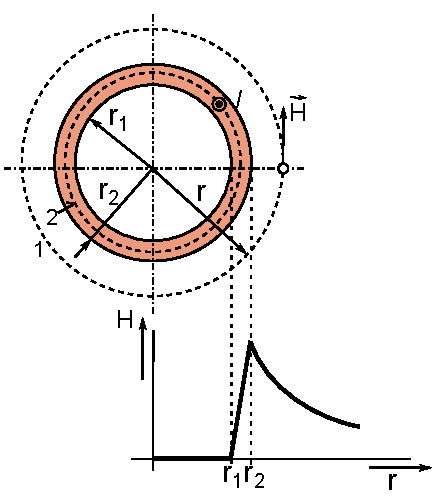
\includegraphics[width=0.4\textwidth]{duf_duty_valec_H.pdf}
        \caption[Pole dlouhého dutého válcového vodiče]{K příkladu stanovení intenzity magnetického
                 pole dlouhého dutého válcového vodiče protékaného proudem}
        \label{TEMP:fig_pole_duty_valec}
      \end{figure}

      Vodič s rovnoměrně rozloženým proudem podle obr. \ref{TEMP:fig_pole_duty_valec} je rotačně
      souměrný podle své osy a tedy i jeho magnetické pole je souměrné. Silové čáry jsou soustředné
      kružnice, vektor $\vr{H}$, jenž má směr tečny ke kružnici, je po celé délce kružnice stejně
      velký. Lze tedy snadno použít integrálního tvaru 1. MR (\textbf{zákon celkového proudu})

      Pro body ležící vně vodiče obepíná kruhová integrační dráha (vedená po silové čáře 1) celý
      proud vodiče $I$ a platí
      \begin{equation}\label{TEMP:eq_1MR_duty_valec}
        \oint_\mathcal{C}\vr{H}d\vr{l} = H\cdot 2\pi r = I
      \end{equation}
      takže intenzita pole je
      \begin{equation}\label{TEMP:eq_H_duty_valec}
        H = \frac{I}{2\pi r}
      \end{equation}

      Ve stěně dutého magnetického vodiče jsou silové čáry rovněž kružnice, neboť magnetické pole
      je i zde souměrné. Tyto siločáry však obepínají jen část proudu $I'$ vodiče pro oběh siločáry
      2 platí
      \begin{equation}\label{TEMP:eq_1MR_uvnitr_valce}
        \oint_\mathcal{C}\vr{H}d\vr{l} = H\cdot 2\pi r = I' = \pi(r^2-r_1^2)J
      \end{equation}
      kde $J$ je hustota proudu ve vodiči
      \begin{equation}\label{TEMP:eq_J_duty_valec}
        J = \frac{I}{S}= \frac{I}{\pi(r_2^2-r_1^2)}
      \end{equation}
      Ve stěně vodiče je tedy intenzita pole
      \begin{equation}\label{TEMP:eq_H_uvnitr_valce}
        H = \frac{I}{2\pi r}\frac{r^2-r_1^2}{r_2^2-r_1^2}
      \end{equation}
      V dutině vodiče je intenzita rovna nule. Vzhledem k souměrnosti pole by i zde muselo platit
      $\oint_\mathcal{C}\vr{H}d\vr{l} = H\cdot 2\pi r$. Protože dráha s poloměrem $r<r_1$ neobepíná
      žádný proud, je $\oint_\mathcal{C}\vr{H}d\vr{l} = 0$ a tedy musí byt $H = 0$.
      \end{example}    
      
      %---------- Example --------------
      \begin{example}\label{TEMP:ex_koax_H}
        Stanovote intezitu magnetického pole dlouhého přímého sousého kabelu podle obr.
        \ref{TEMP:fig_exam_koax_nacrt}. Středním vodičem (\emph{žílou}) prochází proud $I$ a týž
        proud opačného smyslu prochází vnějším vodičem (\emph{pláštěm}). Proudy jsou rovnoměrně
        rozloženy po průřezech vodičů. Nakreslete graf průběhu $H = f(r)$ \cite[s.~92]{Dufek1970},
        \cite[s.~195]{Kotlan1999}.
        
         \begin{figure}[ht!]
           \centering
           \subfloat[Sousý kabel]{\label{TEMP:fig_exam_koax_nacrt}
             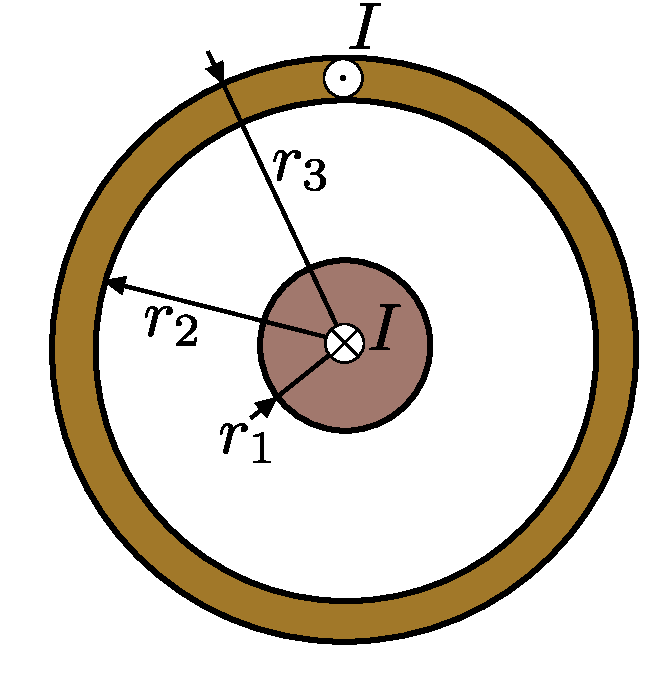
\includegraphics[width=0.2\textwidth]{vypocet_H_sousy_kabel.pdf}}
           \subfloat[Výsledné pole]{\label{TEMP:fig_exam_koax_pole}
             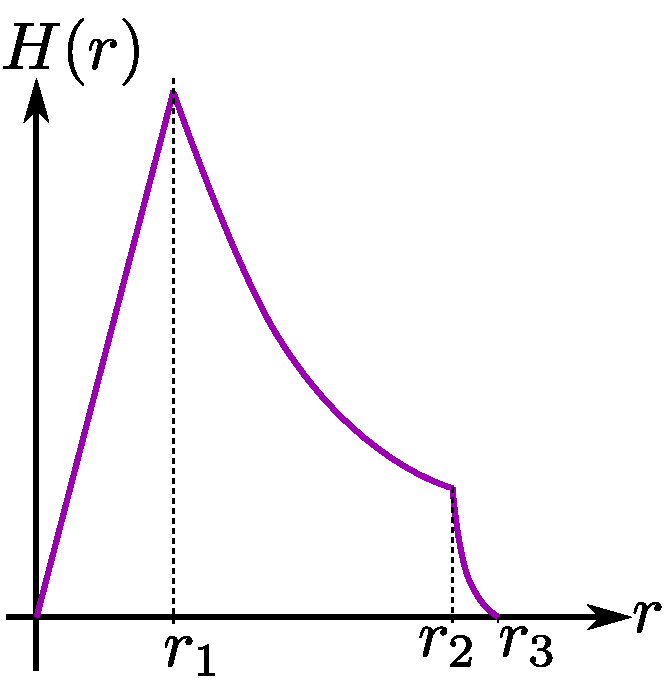
\includegraphics[width=0.2\textwidth]{koax_H_prubeh.pdf}}
           \caption[Pole dlouhého sousého kabelu]{K příkladu stanovení intenzity magnetického pole
                   dlouhého souosého kabelu protékaného proudem: a) náčrt; b) $H=f(r)$}
           \label{TEMP:fig_exam_koax}
         \end{figure}
                 
        
       \textbf{Řešení}: Rovnici \ref{TEMP:eq_1MR_v_hom_p} aplikujeme na jednotlivé intervaly osově
        souměrného starionárního magnetického pole, přičemž se prakticky jedná o superpozici dvou
        polí. V oblasti $r<r_2$ se uplaťnuje pouze pole vnitřního válcového vodiče (žíly), pro
        $r>r_2$ přistupupje sousosé pole vnějšího trubkového vodiče.
        \begin{itemize}
  		  \item Pro oblast $r<r_1$ je vzhedem k 
  		       \begin{align*}
				% \nonumber to remove numbering (before each equation)
				  dI   &= \vr{J}d\vr{S} \\
  				  I(r) &= \int_S dI = \int_S \vr{J}d\vr{S} = \int_S J\cos\beta dS \\
  				       &= \left|\begin{array}{cc}
                                  \beta = 0 & H = \text{konst} \\
                                  S = \pi r^2 & dS = 2\pi rdr \\
                                \end{array}\right| = J\int_0^r 2\pi rdr = J\pi r^2
			   \end{align*}
	 		   hledané řešení 1. MR dáno 
	 		   $$\oint_\mathcal{C}\vr{H}d\vr{l} = H_1 2\pi r = I(r) = J\pi r^2$$ kde celková proudová
	 		   hustota je  $$J = \frac{I}{\pi r_1^2}$$ a tedy $$H_1 = \frac{I}{2\pi r_1^2}\cdot r$$
			   
  		  \item Pro oblast $r_2>r>r_1$ řešíme v podstatě pole vně osamoceného válcového vodiče
  		        $I(r)$ a tedy $$H_2 = \frac{I}{2\pi r}$$
  		  \item Pro $r>r_3$ je magnetické pole vytvářeno celým proudem žíly $I$ a příslušnou částí
  		        proudu pláště $J\pi(r^2 - r_2^2)$, kde prouduová hustota $$J =
  		        \frac{I}{\pi(r_3^2-r_2^2)}$$ má opačnou orientaci oproti proudové hustotě žíli.
  		  
  		  Pak 
  		   \begin{align*}
			 I(r)                           &= I - I\frac{r^2-r_2^2}{r_3^2-r_2^2} \\
			 \oint_\mathcal{C}\vr{H}d\vr{l} &= H_32\pi r = I(r)                   \\				  
			 H_3                            &= \frac{I}{2\pi r}\left(1 - 
			                                   \frac{r^2 - r_2^2}{r_3^2 - r_2^2}\right) 
		   \end{align*}
		  Stejný výsledek dostaneme superpozicí opačně orientovaných polí $$H_3 = H'_3 - H''_3 =
		  \frac{I}{2\pi r} - \frac{I}{2\pi r}\left(\frac{r^2 - r_2^2}{r_3^2 - r_2^2}\right)$$. 
        \end{itemize}
        Pruběh $H(r)$ je na obr. \ref{TEMP:fig_exam_koax_pole}.
      \end{example}

    % -----------Magnetické pole elektrického proudu v diferenciálním tvaru-------------------------
    \subsection{Magnetické pole elektrického proudu v diferenciálním tvaru}
      Nechť je opět magnetické pole vyvoláno konstantním el. proudem $I = \text{konst}$. Jak
      vyplývá z předchozí kapitoly, základním vztahem pro toto pole je \emph{Ampérův zákon}
      $$\oint_\mathcal{c}\vr{H_c}d\vr{l} = I$$  Zvolme za integrační dráhu $c$ obvod malé plošky
      $\Delta S$, jíž prochází proud $\Delta I = J_n \Delta S$, kde $J_n$ je průmět vektoru hustoty
      proudu do směru normály plošky $\Delta S$ (předpokládáme, že ploška $\Delta S$ je dostatečně
      malá, aby se dalo počítat s konstantní hustotou proudu v celém jejím rozsahu)
      \cite[s.~13]{Trnka1972}. Pro zvolený případ platí
      
      \begin{equation}\label{TEMP:eq_amp_z1}
        \oint_\mathcal{c}\vr{H_c}d\vr{l}  =
           J_n \Delta S \rightarrow \frac{1}{\Delta S}\oint_\mathcal{c}\vr{H_c}d\vr{l} = J_n
      \end{equation} 
      
      Pro $\Delta S \rightarrow 0$ zavedeme označení 
      \begin{equation}\label{TEMP:eq_amp_z2}
        \rot{H}  = \frac{1}{\Delta S}\oint_\mathcal{c}\vr{H_c}d\vr{l}  = J_n
      \end{equation}
      
      Rovnice \ref{TEMP:eq_amp_z2} říká, že \emph{rotace vektoru} $\vr{H}$, ($\rot{H}$), jehož
      průmět do určitého směru je roven průmětu vektoru hustoty proudu do tohoto směřu. Z uvedených
      vztahu je patrný fyzikální význam rotace vektoru $\vr{H}$. Je to vektor, jehož velikost je
      rovna oběhovému magnetickému napětí po dráze v rovině kolmé k vektoru hustoty proudu,
      vztaženém k ploše obepínané oběhovou drahou (v nehomogenní poli to platí pro případ, že se
      plocha dráhy blíží k nule).
      
      Při použití pravoúhlé soustavy kartézských souřadnic $x$, $y$ a $z$ jsou průměty vektoru
      $\rot{H}$ do jednotlivých os
      \begin{equation}\label{TEMP:eq_amp_z3}
        \textsf{rot}_x\mathbf{H} = J_x, \qquad 
        \textsf{rot}_y\mathbf{H} = J_y, \qquad
        \textsf{rot}_z\mathbf{H} = J_z
      \end{equation}      
      Průmět $\textsf{rot}_x\mathbf{H}$ je dán oběhovým magnetickým napětím po obvodu plošky $dydz$
      a platí
      \begin{align}\label{TEMP:eq_amp_z4}
        \textsf{rot}_x\mathbf{H} 
          &= \frac{1}{dydz}\oint_\mathcal{c}\vr{H_c}d\vr{l}                             \\ \nonumber
          &= \frac{1}{dydz}\left[H_ydy + \left(H_z + \pder{Hz}{y}dy\right)dz\right] -   \\ \nonumber
          &- \frac{1}{dydz}\left[\left(H_y - \pder{Hy}{z}dz\right)dy - H_zdz\right]     \\ \nonumber
          &= \frac{1}{dydz}\left[\pder{Hz}{y}dydz - \pder{Hy}{z}dydz\right] = 
             \pder{Hz}{y} - \pder{Hy}{z} = J_z
      \end{align}       
      
      \begin{figure}[ht!]
        \centering
        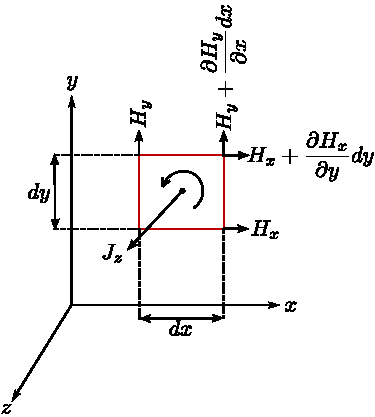
\includegraphics[width=0.8\linewidth]{rotH_dxdy.pdf}
        \caption[K odvození pojmu $\textsf{rot}_z\mathbf{H}$]{K odvození pojmu
                 $\textsf{rot}_z\mathbf{H}$}
        \label{TEMP:fig_rotH_dxdy}
      \end{figure}            
      tedy dostáváme
      \begin{align}\label{TEMP:eq_amp_z5}
        \textsf{rot}_x\mathbf{H} &= \pder{H_z}{y} - \pder{H_y}{z} = J_x      \\ \nonumber
        \textsf{rot}_x\mathbf{H} &= \pder{H_x}{z} - \pder{H_z}{x} = J_y      \\ \nonumber
        \textsf{rot}_x\mathbf{H} &= \pder{H_y}{x} - \pder{H_x}{y} = J_z            
      \end{align}        
      Pro \emph{pravoúhlé souřadnice} $x, y, z$ můžeme tedy vztah $\rot{H} = \vr{J}$ rozepsat na
      tvar
      \begin{align}\label{TEMP:eq_amp_z6}
        \textsf{rot}\mathbf{H} 
          &= \vr{i}\,\textsf{rot}_x\mathbf{H} + \vr{j}\,\textsf{rot}_y\mathbf{H} +
             \vr{k}\,\textsf{rot}_z\mathbf{H} \\ \nonumber &= \vr{i}\left(\pder{H_z}{y} -
             \pder{H_y}{z}\right) +  \vr{j}\left(\pder{H_x}{z} - \pder{H_z}{x}\right) +
             \vr{k}\left(\pder{H_y}{x} - \pder{H_x}{y}\right)                           \\ \nonumber 
          &= \vr{i}\,J_x + \vr{j}\,J_y + \vr{k}\,J_z = \vr{J}.
      \end{align}          
      
      Rotaci vektoru $\rot{H}$ můžeme též symbolicky vyjádřit vektorovým součinem Hamiltonova
      operátoru a vektoru $\vr{H}$
      \begin{equation}\label{TEMP:eq_amp_z7}
        \rot{H}  = \nabla\times\vr{H} = \left(\vr{i}\,\pder{ }{x} + 
                   \vr{j}\,\pder{ }{y} + \vr{k}\,\pder{ }{z}\right)\times(\vr{i}\,H_x +
                   \vr{j}\,H_y + \vr{k}\,H_z)
      \end{equation}         
      nebo také determinantu
      \begin{equation}\label{TEMP:eq_amp_z8}
        \rot{H} = \begin{vmatrix}
                    \vr{i}       & \vr{j}      & \vr{k}      \\
                    \pder{ }{x}  & \pder{ }{y} & \pder{ }{z} \\ 
                    H_x          & H_y         & H_z         \\
                  \end{vmatrix}      
      \end{equation}  
      \begin{minipage}[t]{0.4\textwidth}% first column                  
        \emph{cylindrických souřadnic} $r$, $\varphi$, $z$:
        \begin{align}\label{TEMP:eq_amp_z9}
          \textsf{rot}_r\mathbf{H}       
            &= \frac{1}{r}\pder{H_z}{\varphi} - \pder{H_\varphi}{z} = J_r          \\ \nonumber 
          \textsf{rot}_\varphi\mathbf{H} 
            &= \pder{H_r}{z} - \pder{H_z}{r}                        = J_\varphi    \\ \nonumber
          \textsf{rot}_z\mathbf{H}       
            &= \frac{1}{r}\left[\pder{ }{r}
               \left(rH_\varphi\right)-\pder{H_r}{\varphi}\right]   = J_z                                  
        \end{align} 
      \end{minipage}
      \begin{minipage}[t]{0.6\textwidth}% second column
        \emph{sférických souřadnic} $r$, $\varphi$, $\vartheta$ 
        \begin{align}\label{TEMP:eq_amp_z10}
          \textsf{rot}_r\mathbf{H}        
             &= \frac{1}{r\sin\vartheta}\left[\pder{ }{\vartheta}(H_\varphi\sin\vartheta) - 
                \pder{H_\vartheta}{\varphi}\right]                     = J_r          \\  \nonumber 
          \textsf{rot}_\varphi\mathbf{H}   
             &= \frac{1}{r}\left[\pder{ }{r}(rH_\vartheta) - 
                \pder{H_r}{\vartheta}\right]                           = J_\varphi    \\  \nonumber
          \textsf{rot}_\vartheta\mathbf{H} 
             &= \frac{1}{r\sin\vartheta}\left[\pder{H_r}{\varphi} -
                \pder{ }{r}\left(rH_\varphi\sin\vartheta\right)\right] = J_\vartheta    
      \end{align} 
      \end{minipage}
      Podobně jako v elektrickém poli vyjadřujeme vztah $\oint\vr{D}d\vr{S} = Q$ vztahem $\diver{D}
      = \rho$, tak i v magnetickém poli vyjadřujeme vztah $\oint\vr{B}d\vr{S} = 0$ vztahem
      $\diver{D} = 0$, nebo též v kartézských souřadnicích $x$, $y$ a $z$ jako $$\diver{D} =
      \nabla\cdot\vr{B} = \pder{B_x}{x} + \pder{B_y}{y} + \pder{B_z}{z} = 0$$
                     
    % ----------------Rovnice pro magnetický potenciál----------------------------------------------
    \subsection{Rovnice pro magnetický potenciál}
      V regulárních bodech lineárního homogenního izotropního magnetika platí pro $\varphi_m$
      \textbf{Laplaceova rovnice}
      \begin{equation}\label{TEMP:eq_varphi_m_laplace}
        \Delta\varphi_m = 0
      \end{equation}      
    Důkaz plyne z rovnice $\diver{B} = 0$ a rovnice $\vec{B} = \mu\vec{H}$: $$\diver{B} =
    \textsf{div}\mu\vec{H} = \textsf{div}\mu(-\textsf{grad}\varphi_m).$$ Pro $\mu = \text{konst}$
    dostáváme $\textsf{div}\textsf{grad}\varphi_m = 0$, což je rovnice
    \ref{TEMP:eq_varphi_m_laplace}.
    
    Na rozhraní mezi dvěma magneticky různými prostředími neplatí Maxwellovy rovnice v
    diferenciálním tvaru a tedy ani Laplaceova rovnice \ref{TEMP:eq_varphi_m_laplace}. Podmínky pro
    $\vr{H}$ a $\vr{B}$ na rozhraní vyjádříme pomocí skalárního magnetického potenciálu
     \begin{align}\label{TEMP:eq_mag_U_rozhrani}
       \varphi_{m1}                 &= \varphi_{m2} \\
       \mu_1\pder{\varphi_{m1}}{n}  &= \mu_2\pder{\varphi_{m2}}{n} 
     \end{align}
    kde $\pder{}{n}$ jsou derivace ve směru normály k rozhraní. 
    
    \subsubsection{Vektorový magnetický potenciál}
      V elektrostatice jsme pro usnadnění mnohých problémů zavedli skalární elektrický potenciál -
      lze jej zavést vždy, neboť elektrostatické pole je vždy potenciální. Magnetické pole je však
      obecně vírové. Lze jej popsat skalárním potenciálem jen ve speciálních případech, tj.
      jestliže je polem potenciálním. Obecně je však zavedení skalárního potenciálu nepřípustné.
      Lze i pak zavést nějakou veličinu (analogickou skálárnímu potenciálu), s níž by se pracovalo
      snáze, než přímo s vektory pole?
      
      Dříve než definujeme vektorový magnetický potenciál, zopakujme zavedení skalárního potenciálu
      v elektrostatice. Vyjďeme z 2. MR a z rovnice známé z vektorové analýzy: $$\rot{E} = 0 \qquad
      \text{a} \qquad \textsf{rot}\,\textsf{grad}\varphi_m = 0.$$
      
      V magnetickém poli vyjdeme ze 4. MR a z jiné identity pro vektorovou funkci $\vr{A}$, známe z
      vektorové analýzy: $$\diver{B} = 0 \qquad \text{a} \qquad \textsf{div}\textsf{rot}\vec{A} =
      0$$ odtud
        \begin{equation}\label{TEMP:eq_B_rotA}
          \vec{B} = \rot{A}.
        \end{equation}       
               
\printbibliography[heading=subbibliography]          